\section{Beyond One Setting: Architecture, Attack, and Trigger Knowledge}
\label{sec:general}

\subsection{The Cliff Transfers}
Table~\ref{tab:e7} repeats the critical cells on three settings: VGG-16-BN with
BadNets, VGG-16-BN with Blend, and ResNet-18 with Blend. ResNet-18/BadNets is
already covered by the grid. In every setting, deletion at recall 0.75 or 0.5
fails completely: ASR is 99.42--100.00\% and clean accuracy is indistinguishable
from gold. In every setting, the recipe at the same recall holds ASR at or below
$1.02\%$. The largest clean-accuracy cost is 4.09 points, in the VGG-16-BN/Blend
cell at $r{=}0.5$ ($84.80\%$ against a gold of $88.89\%$); VGG-16-BN/BadNets
costs 3.26 points at the same recall. ResNet-18 is cheaper: 2.60 points for
Blend at $r{=}0.75$ and 2.04 points at $r{=}0.5$. The recipe is thus not free, and its cost grows with the
depth of the architecture and the strength of the trigger, but it remains inside
a plausible budget where deletion is not.

Fig.~\ref{fig:e7} shows the same cells on a log scale. Panel (a) separates the
two outcomes: every deletion cell is at 99.42--100.00\%, more than an order of
magnitude above the 5\% line, while every recipe cell is at 0.29--1.02\%. Panel
(b) is the price. Deletion is within 0.7 points of gold in every cell, because
the poison it fails to remove also does not change clean accuracy at this scale.
The recipe's cost is ordered by trigger strength first and depth second: 1.71 and
3.26 points for VGG-16-BN/BadNets at $r{=}0.75$ and $0.5$; 2.99 and 4.09 for
VGG-16-BN/Blend; 2.60 and 2.04 for ResNet-18/Blend. The cost exceeds three points
at $r{=}0.5$ on VGG-16-BN for both attacks (3.26 points with BadNets and 4.09
with Blend).

\begin{figure}[t]
\centering
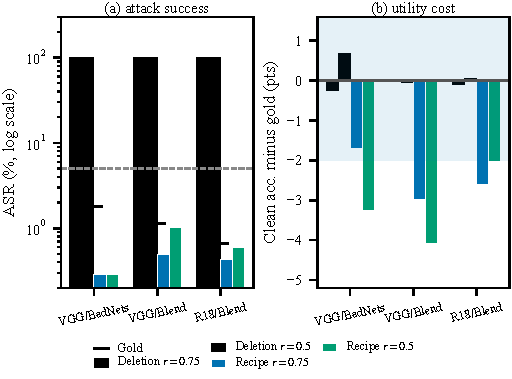
\includegraphics[width=\columnwidth]{fig17_e7_transfer.pdf}
\caption{The transfer settings. (a) ASR after deletion and after the recipe at
recall 0.75 and 0.5, on a log scale; the dashed line is 5\%. (b) Clean accuracy
relative to each setting's gold model; the shaded band is the two-point budget.
Deletion stays within 0.7 points of gold and does not remove the backdoor; the
recipe removes it at a cost of 1.7--4.1 points.}
\label{fig:e7}
\end{figure}

The transfer matters because the cliff could have been an artefact of one
architecture's optimisation. It is not. The step appears in a network with batch
normalisation at every layer and in one with a different depth and width, under a
local patch trigger and under a global blend trigger. The location of the step
does not move: it lies between full removal and partial removal at 75\%,
consistent with the E1 boundary between 95\% and 90\% recall.

\begin{table}[t]
\centering
\caption{E7: the cliff and the recipe's tolerance transfer across architecture and attack.}
\label{tab:e7}
\footnotesize
\setlength{\tabcolsep}{4pt}
\begin{tabular}{lccc}
\toprule
\textbf{Method} & \shortstack{\textbf{VGG-16-BN}\\\textbf{BadNets}} & \shortstack{\textbf{VGG-16-BN}\\\textbf{Blend}} & \shortstack{\textbf{ResNet-18}\\\textbf{Blend}} \\
\midrule
Gold & 88.95 / 1.80 & 88.89 / 1.14 & 88.75 / 0.66 \\
Deletion, $r{=}0.75$ & 88.71 / 100.00 & 88.93 / 99.42 & 88.64 / 99.70 \\
Deletion, $r{=}0.5$ & 89.64 / 100.00 & 88.83 / 99.84 & 88.81 / 99.94 \\
Recipe, $r{=}0.75$ & 87.24 / 0.29 & 85.90 / 0.49 & 86.15 / 0.43 \\
Recipe, $r{=}0.5$ & 85.69 / 0.29 & 84.80 / 1.02 & 86.71 / 0.60 \\
\bottomrule
\end{tabular}
\par\vspace{1pt}\footnotesize\raggedright Cells are clean accuracy / ASR (\%). Gold is the oracle retrain at $r{=}1$. Deletion fails at both recall levels for every architecture--attack pair; the recipe holds ASR $\leq1.02\%$, at a clean-accuracy cost of up to 4.09 points at $r{=}0.5$.
\end{table}


\subsection{The Recipe's Tolerance Is Bought With Trigger Knowledge}
The recipe's advantage comes from its inoculation stage, which presents the
trigger to the network with the correct label. That step requires the trigger. In
the grid, and in Table~\ref{tab:e7}, the true trigger is used. This is a
known-trigger upper bound, and it is essential to say so: a defence that must be
told the trigger is not a blind defence, and a practitioner who does not know the
trigger cannot run the recipe in the form that produces these numbers.

To measure how much the bound is worth, we replace the true trigger with one
synthesised from the poisoned model by the Neural Cleanse procedure described in
Section~\ref{sec:methods}. Table~\ref{tab:e7b} reports the result. On
ResNet-18/BadNets the synthesised mask has zero intersection with the true
$4\times4$ patch (IoU $=0.000$), and inoculation with it leaves ASR at
$98.99\%$ with clean accuracy $87.67\%$. On ResNet-18/Blend the synthesised mask
has a soft mass of about 166 pixels, roughly ten times the 16 pixels of the true
patch, and inoculation with it leaves ASR at $95.72\%$ with clean accuracy
$87.32\%$. In other words, the synthesis stage recovers a mask that is large and
diffuse, not the compact patch that the attack uses, and the inoculation built on
it does not remove the backdoor.

This is the strongest negative result in the paper, because it closes the obvious
escape route. One might hope that a defence could use the recipe's tolerance
without knowing the trigger, by synthesising the trigger first. On these two
attacks, that composition fails at the first step. The recipe is therefore best
read as a ceiling: it shows what trigger-aware repair can achieve under imperfect
recall, and it bounds from above what any trigger-synthesis-based defence could
achieve if synthesis were perfect. It does not demonstrate a deployable method.

\begin{table}[t]
\centering
\caption{E7b: replacing the true trigger with a synthesised one destroys the
recipe's advantage.}
\label{tab:e7b}
\footnotesize
\begin{tabular}{lcccc}
\toprule
\textbf{Setting} & \textbf{Clean} & \textbf{ASR} & \textbf{IoU} & \textbf{Mask mass} \\
\midrule
R18/BadNets & 87.67 & 98.99 & 0.000 & -- \\
R18/Blend & 87.32 & 95.72 & -- & 166 \\
\bottomrule
\end{tabular}
\par\vspace{1pt}\footnotesize\raggedright Inoculation with a synthesised trigger,
recall 1.0. The true BadNets patch occupies 16 pixels; the synthesised Blend mask
has a soft mass of 166 pixels, about ten times larger. With the true trigger the
recipe holds ASR at $0.63\%$ on ResNet-18/BadNets at $r{=}1$
(Table~\ref{tab:e1grid}) and at $0.43$--$0.60\%$ on ResNet-18/Blend at
$r{=}0.75$ and $0.5$ (Table~\ref{tab:e7}). IoU and mask mass were not both logged
for every cell; the table reports what each run recorded.
\end{table}

\subsection{Which Component Does the Work?}
The E1 grid contains an inoculation-only baseline ($17.67\%$ ASR) and the E8
block contains a label-repair-only baseline ($8.63$--$16.36\%$ ASR, discussed in
Section~\ref{sec:calib}). Neither alone crosses the 5\% threshold; the
combination does, at $0.63$--$2.95\%$ across the grid. The two stages are
complementary rather than redundant. Repair removes the label noise that would
otherwise teach the network to associate the trigger with the target; inoculation
changes the association even for poison that never entered the forget set. The
first is bounded by recall, the second is bounded by trigger knowledge. The
recipe works in the middle ground where each covers the other's weakness.

This decomposition also explains why the recipe degrades gracefully rather than
catastrophically. At $r{=}0.5$, half the poison is still in the training set,
but its labels have been repaired (for the half that was flagged) and the trigger
has been re-labelled for the whole network through inoculation. The residual
association is weak, and ASR sits at 2--4\% rather than at 100\%. At $r{=}0.25$
the repair covers too little of the poison for the inoculation to dominate, and
ASR rises to 5.42\%. The transition is gradual because it reflects a balance
between two mechanisms, not a threshold in the data.

\subsection{Poison Rate}
The amplification study (Section~\ref{sec:calib}) runs at a 10\% poison rate and
therefore provides a second scale. At that rate, a partial label repair without
inoculation lowers ASR from 99.99\% to between 11.07\% and 33.03\% depending on
seed and strength. That is a substantial reduction, but it is not a removal by
our criterion, and it occurs in a regime where the detector itself is weakest:
activation clustering returns no flags at 10\%, and spectral signatures recovers
48.0\% of the poison. The combination of a harder attack and a worse detector is
exactly the regime in which a controlled study is most useful, because it is
where the difference between a method that needs recall and a method that does
not becomes visible. We do not claim that the recipe's tolerance is
rate-independent; the 10\% block does not include the full recipe, and we did not
run the full grid at 10\%.
